\documentclass[tikz, convert={outfile=\jobname.svg}]{standalone}
\usetikzlibrary{arrows, positioning, quotes}
\begin{document}
	% \tikz [every node/.style={draw}] \graph[layered layout]{
	% 	% GCS/"Ground Control Station" <-> Platform/"Flight Platform";
	% 	Antenna -> RF/"LNA";
	% 	SDR <- RF;
	% 	Sensors/"GPS/Compass" -> Joule/"On Board Computer";
	% 	Joule <- SDR;
	% 	UI <-> Joule;
	% 	Storage/"Data Storage" <- Joule;
	% };

	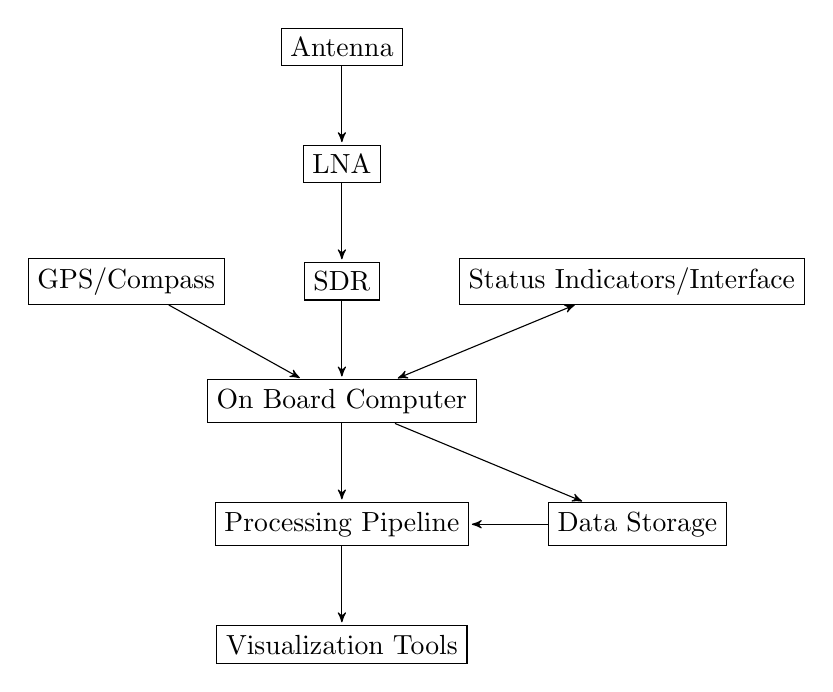
\begin{tikzpicture}[
						block/.style={draw,rectangle},
						every label/.append style={font=\tiny},
						every edge/.append style={draw, -stealth', shorten > = 1pt, font=\footnotesize, inner sep = 2pt, auto, align=left},]
		\node (ant) [block] {Antenna};
		\node (lna) [block, below=of ant] {LNA};
		\node (sdr) [block, below=of lna] {SDR};
		\node (gps) [block, left=of sdr] {GPS/Compass};
		\node (ui) [block, right=of sdr] {Status Indicators/Interface};
		\node (obc) [block, below=of sdr] {On Board Computer};
		\node (sigproc) [block, below=of obc] {Processing Pipeline};
		\node (data) [block, right=of sigproc] {Data Storage};
		\node (viz) [block, below=of sigproc] {Visualization Tools};


		\path 	(ant) 		edge 	(lna)
				(lna) 		edge 	(sdr)
				(sdr)		edge	(obc)
				(gps)		edge	(obc)
				(ui)		edge[stealth'-stealth']	(obc)
				(obc)		edge	(data)
				(obc)		edge	(sigproc)
				(data)		edge	(sigproc)
				(sigproc)	edge	(viz);
	\end{tikzpicture}

\end{document}